We tested our strategies on two different simulations, Lulesh and CloverLeaf3D. 
%
For each simulation we measured the average NRMSE compared to the original data and compared our results with standard compression. 
%
We also measured the overhead of our strategies. 
\begin{comment}
\vspace{-1.3em}
\subsection{Lulesh}
Lulesh takes time to advance to an interesting state, so for the majority of the cycles only rank 0 has pertinent data.
%
Thus, the reallocation strategies were able to devote their entire I/O budget to saving rank 0's data, whereas the standard compression would only save a fixed portion of rank 0's data. 
%
Moreover, by dedicating the entire I/O budget to rank 0, the reallocation strategies saved out less data overall than the standard compression. 
%
This is due to the fact that rank 0's total data size is smaller than the total budget (i.e. $120^3 < \frac{1000^3}{128} < \frac{1000^3}{64} < \frac{1000^3}{32}$).  

The results in Table~\ref{table:results} demonstrates that the disproportionate makeup of the data heavily favored our reallocation strategies, which improved on standard compression by several orders of magnitude. 
%
Figure~\ref{fig:lulesh} shows the visual artifacts present in the standard compression.
%
Here, our reallocation strategies prioritized this data in order to save a more accurate representation of the original data compared to the standard compression. 

\begin{figure}[h!]
  \centering
  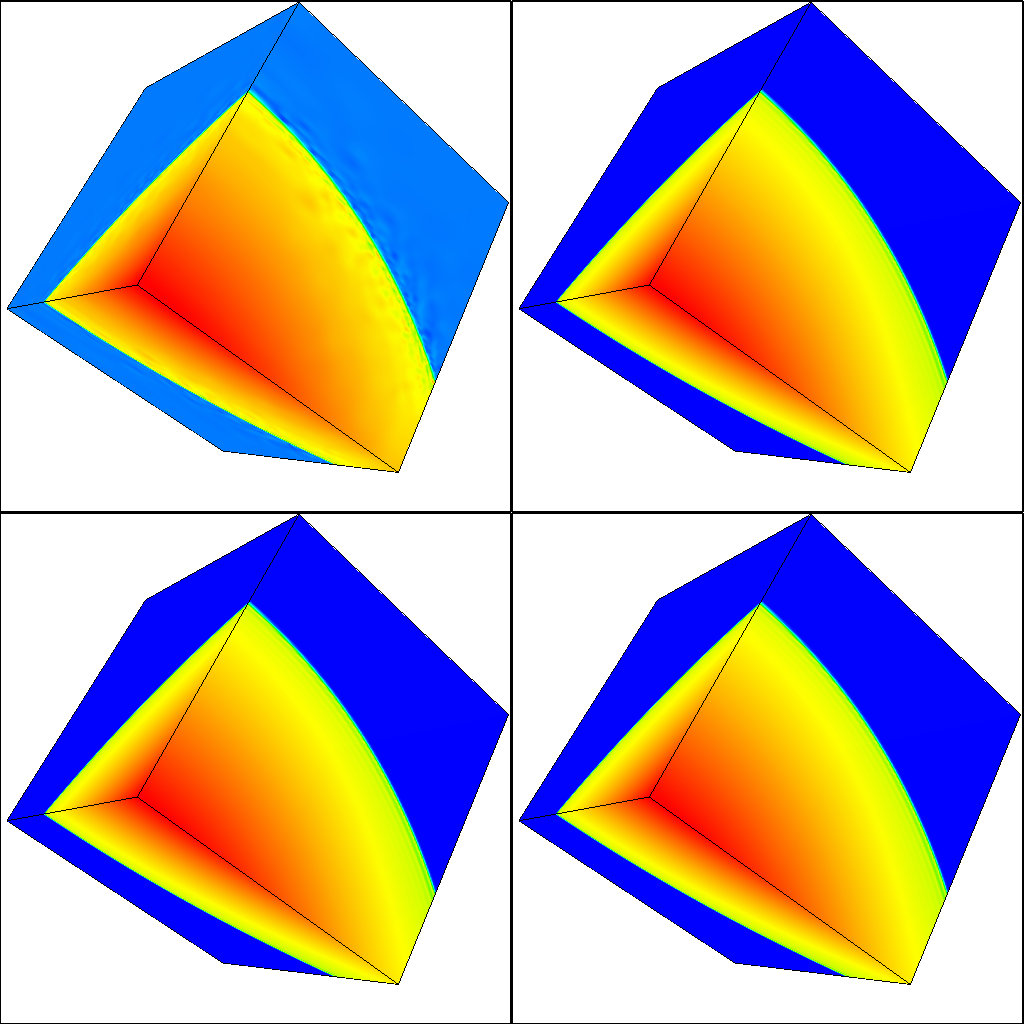
\includegraphics[scale=0.13]{images/lulesh128.png}
  \caption{\textbf{Top Left:} The standard compression using 128:1 compression ratio. \textbf{Top Right:} Reallocation strategy based on magnitude. This strategy determined the data should be saved using a 7:1 compression ratio. \textbf{Bottom Left:} The original data. \textbf{Bottom Right:} Reallocation strategy based on entropy. This strategy determined the data should be saved using a 3:1 compression ratio. }
  \label{fig:lulesh}
\end{figure}

\begin{table}[t]
\begin{tabular}{|l|l|l|l|}
\hline
 \makecell{Compression \\ Ratio} & \makecell{Standard\\ Avg.\\ NRMSE} &\makecell{ Magnitude\\ Avg.\\ NRMSE} & \makecell{Entropy\\ Avg.\\ NRMSE} \\ \hline
\makecell{32:1} & 0.00055 & 3.73E-13  & 3.97E-08  \\ \hline
\makecell{64:1} & 0.00184  & 4.58E-09  & 9.58E-08  \\ \hline
\makecell{128:1} & 0.00436  & 9.32E-06  & 4.98E-07  \\ \hline
\end{tabular}
\caption{The average NRMSE for the reallocation strategies for each I/O budget on Lulesh.}
\label{table:results}
\end{table}
\vspace{-1.0em}

\vspace{-1.3em}
\subsection{CloverLeaf3D}
CloverLeaf3D advances to an interesting state more quickly than Lulesh as shown in Figure~\ref{fig:clover}, hence the reduced cycles for the experiment. 

\begin{figure}[h!]
  \centering
  \begin{subfigure}[b]{0.45\linewidth}
    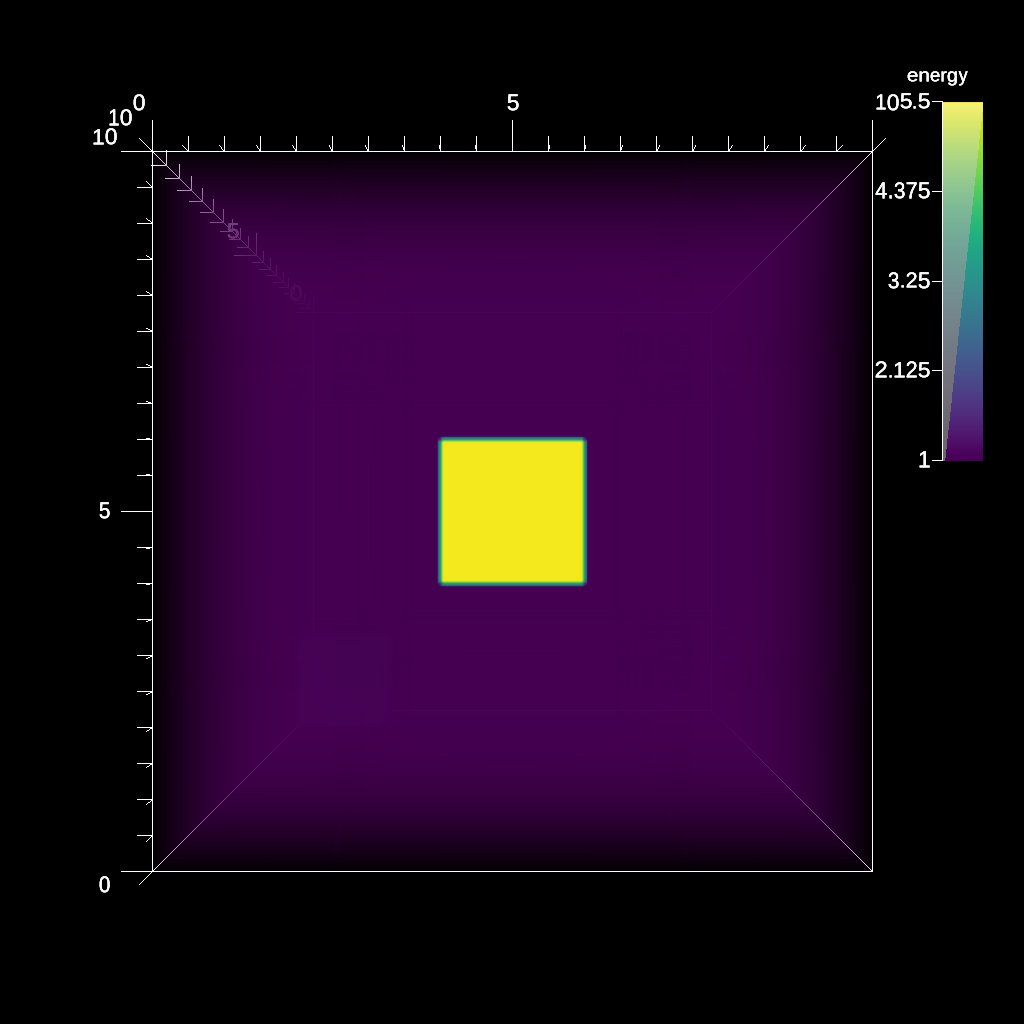
\includegraphics[width=\linewidth]{images/clover1.png}
    \caption{Timestep 10}
  \end{subfigure}
  \begin{subfigure}[b]{0.45\linewidth}
    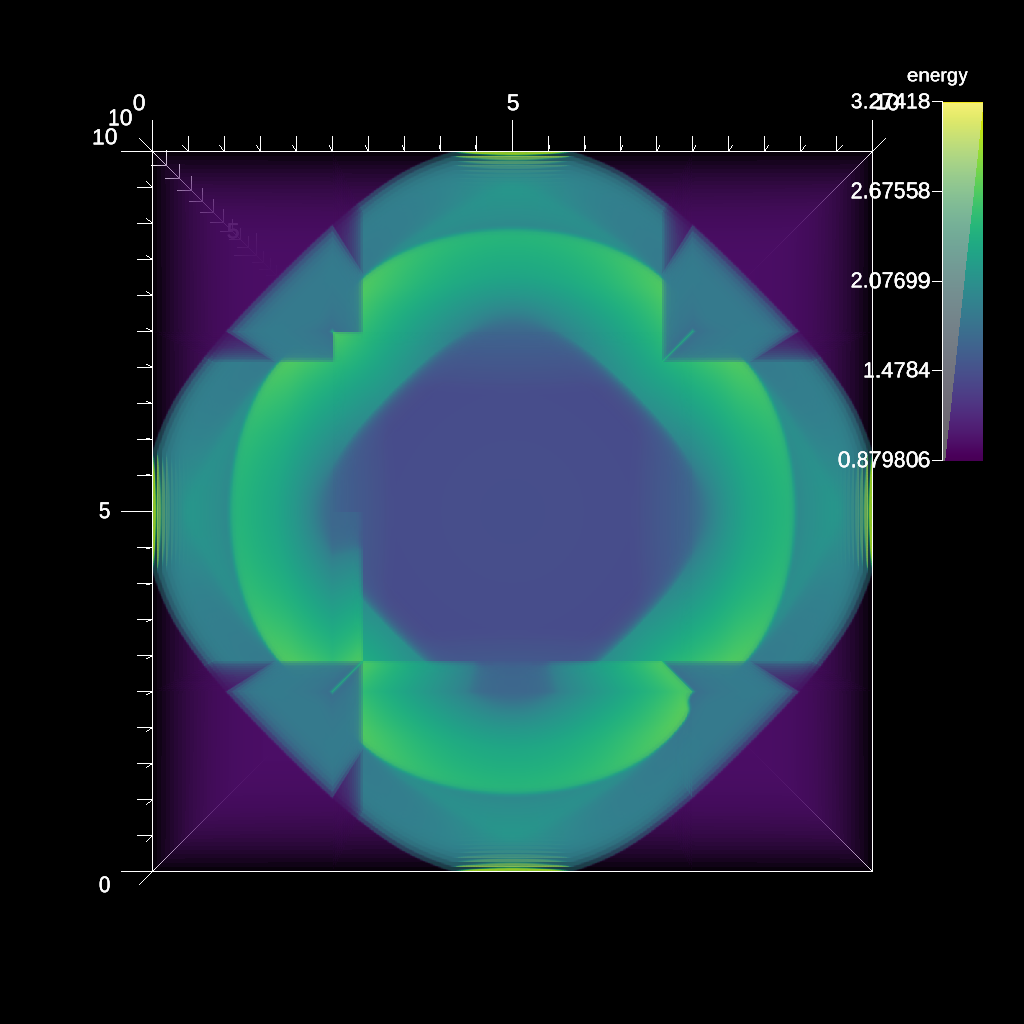
\includegraphics[width=\linewidth]{images/clover2.png}
    \caption{Timestep 63,640}
  \end{subfigure}
  \caption{CloverLeaf3D at (a) the beginning of the simulation and (b) at the of the simulation.}
  \label{fig:clover}
\end{figure}
\end{comment}
The results for CloverLeaf3D in Figure~\ref{fig:clover} shows that all allocation strategies performed similarly as the simulation progressed, but showed information gains during early cycles. 
%
With a more dispersed makeup of important data, the reallocation strategies were similar to the fixed compression ratio in terms of distributing the I/O budget.


Similar to Lulesh, the reallocation strategies attained increased I/O savings during the early cycles when the data was more condensed and only several ranks were saving out their entire slice of data.
%
However, those savings decreased as the simulation progressed, eventually both reallocation strategies were using the full extent of their I/O budget. 

%\begin{figure}[h!]
%  \centering
%  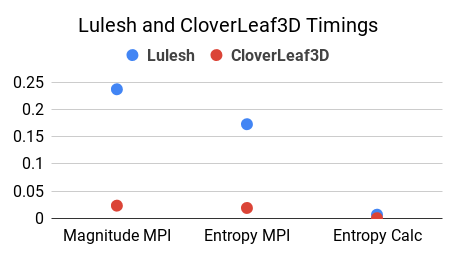
\includegraphics[scale=0.5]{images/timings.png}
%  \caption{The average MPI timing for each strategy and the average time to calculate entropy. }
%  \label{fig:timings}
%\end{figure}




%\begin{table*}[t]
%\begin{tabular}{|l|l|l|l|l|l|l|}
%\hline
%\makecell{Simulation\\ \& \\ Compression Ratio} & \makecell{Standard\\ Avg. NRMSE} & \makecell{Standard\\ Max NRMSE} &\makecell{ Magnitude\\ Avg. NRMSE} & \makecell{Magnitude\\ Max NRMSE} & \makecell{Entropy\\ Avg. NRMSE} & \makecell{Entropy \\Max NRMSE} \\ \hline
%\makecell{Lulesh\\ 32:1} & 0.000546425 & 0.000967242 & 3.73E-13 & 5.59E-09 & 3.97E-08 & 3.24E-07 \\ \hline
%\makecell{64:1} & 0.00183721 & 0.00389347 & 4.58E-09 & 7.95E-07 & 9.58E-08 & 8.35E-07 \\ \hline
%\makecell{128:1} & 0.00435958 & 0.00805588 & 9.32E-06 & 1.39E-05 & 4.98E-07 & 4.31E-06 \\ \hline
%\makecell{CloverLeaf3D\\ 32:1} & 0.0002182 & 0.271049 & 0.000216421 & 0.297249 & 0.000237173 & 0.960391 \\ \hline
%\makecell{64:1} & 0.00250432 & 0.221038 & 0.00220037 & 0.221038 & 0.00196741 & 0.543476 \\ \hline
%\makecell{128:1} & 0.00334693 & 0.221038 & 0.00288031 & 0.239174 & 0.00217648 & 0.251461 \\ \hline
%\end{tabular}
%\caption{The average NRMSE for the reallocation strategies at each compression ratio for Lulesh.}
%\label{table:results}
%\end{table*}

\begin{comment}
\begin{figure}
    \begin{subfigure}[b]{\textwidth}
        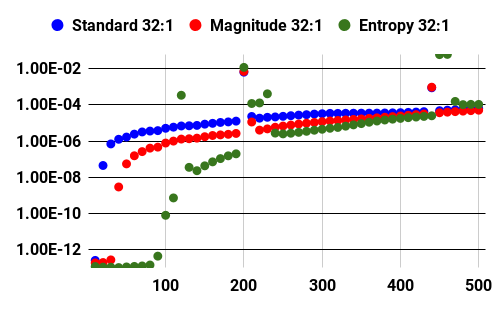
\includegraphics[scale=0.44]{images/clover32.png}
%        \caption{The average RMSE over time for each strategy using compression ratio 32:1}
        \label{fig:32}
    \end{subfigure}
    \begin{subfigure}[b]{\textwidth}
        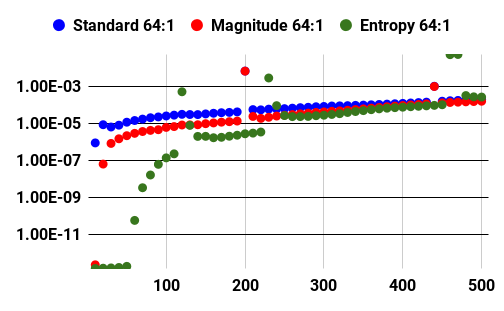
\includegraphics[scale=0.44]{images/clover64.png}
%        \caption{The average RMSE over time for each strategy using compression ratio 64:1}
        \label{fig:64}
    \end{subfigure}
    \begin{subfigure}[b]{\textwidth}
        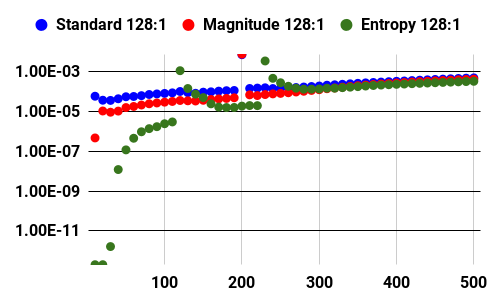
\includegraphics[scale=0.44]{images/clover128.png}
%        \caption{The average RMSE over time for each strategy using compression ratio 128:1}
        \label{fig:128}
    \end{subfigure}
    \caption{The average RMSE over time for each strategy on CloverLeaf3D with each compression ratio.}\label{fig:clover}
\end{figure}
\vspace{-1.0em}

\begin{table}[h]
\begin{tabular}{|l|l|l|l|}
\hline
 \makecell{Simulation} & \makecell{Magnitude\\MPI} &\makecell{Entropy\\MPI} & \makecell{Entropy\\Calc} \\ \hline
\makecell{Lulesh} & 0.2378385 & 0.1733445  & 0.0063935  \\ \hline
\makecell{CloverLeaf3D} & 0.023089  & 0.0188065  & 8.00E-06  \\ \hline
\end{tabular}
\caption{The average MPI timing for each strategy and the average time to calculate entropy. }
\label{table:timings}
\end{table}

\vspace{-1.3em}
\subsection{Timings}
With any in situ analysis it is important to know if the proposed algorithm creates a detrimental overhead to the simulation as a whole. 
%
We measured the time it takes for each rank to calculate entropy as well as the MPI coordination time. 
%
For both simulations we found the MPI coordination and entropy calculation time to be acceptable for in situ analysis as shown in Table~\ref{table:timings}. 

\end{comment}
